% Created 2021-05-14 Fri 16:46
% Intended LaTeX compiler: pdflatex
\documentclass[presentation]{beamer}
\usepackage[utf8]{inputenc}
\usepackage[T1]{fontenc}
\usepackage{graphicx}
\usepackage{grffile}
\usepackage{longtable}
\usepackage{wrapfig}
\usepackage{rotating}
\usepackage[normalem]{ulem}
\usepackage{amsmath}
\usepackage{textcomp}
\usepackage{amssymb}
\usepackage{capt-of}
\usepackage{hyperref}
\usepackage{minted}
\usepackage[utf8]{inputenc}
\usepackage{color}
\usetheme[height=7mm]{Rochester}
\setbeamertemplate{footline}[frame number]
\usecolortheme[accent=red, light]{solarized}
\setbeamercolor{frametitle}{bg=solarizedRebase02,fg=solarizedAccent}
\setbeamercolor{author in head/foot}{bg=solarizedRebase02,fg=solarizedRebase01}
\setbeamercolor{title in head/foot}{bg=solarizedRebase02,fg=solarizedRebase01}
\setbeamercolor{block title}{bg=solarizedRebase0,fg=solarizedRebase02}
\setbeamercolor{block body}{bg=solarizedRebase02,fg=solarizedRebase0}
\setbeamercolor{item}{bg=solarizedRebase02,fg=solarizedAccent}
\beamertemplatenavigationsymbolsempty
\usemintedstyle{manni}
\AtBeginSection[]{
\begin{frame}
\vfill
\centering
\begin{beamercolorbox}[sep=8pt,center,shadow=true,rounded=true]{title}
\Huge\insertsectionhead\par%
\end{beamercolorbox}
\vfill
\end{frame}
}
\usetheme{default}
\author{Sebastian Stabinger, Thomas Hausberger}
\date{SS2021}
\title{Programmaufteilung}
\hypersetup{
 pdfauthor={Sebastian Stabinger, Thomas Hausberger},
 pdftitle={Programmaufteilung},
 pdfkeywords={},
 pdfsubject={},
 pdfcreator={Emacs 27.2 (Org mode 9.4.5)}, 
 pdflang={Ger}}
\begin{document}

\maketitle

\section{Wozu sollte man ein Programm aufteilen?}
\label{sec:orgcd7bc51}
\begin{frame}[label={sec:orgd8802d1}]{Hintergrund}
\begin{itemize}
\item In C und C++ kann man prinzipiell beliebig große Programme in einer
Datei schreiben (das geht nicht in allen Sprachen)
\item Größere Programme schreibt man aber üblicherweise auf mehrere (oft
sehr viele) Dateien aufgeteilt
\begin{itemize}
\item Der Linux Kernel hat aktuell z.B. knapp 60.000 Dateien mit
24.000.000 Zeilen Code
\end{itemize}
\end{itemize}
\begin{block}{Vorteile einer Aufteilung}
\begin{itemize}
\item Einfacheres Zusammenarbeiten mit anderen Programmierern
\item Übersichtlicher
\item Die Compilezeiten verringern sich sehr
\end{itemize}
\end{block}
\end{frame}
\begin{frame}[label={sec:orgc25f9f5},fragile]{Zusammenarbeiten}
 \begin{itemize}
\item Es ist relativ schwierig eine Datei mit mehreren Leuten gleichzeitig
zu bearbeiten
\item Häufig muss man für die Implementierung einer neuen Funktion das
Programm \alert{kurzzeitig in einen ungültigen Zustand bringen} (das
Programm compiliert nicht mehr). Das wäre für andere Beteiligte
relativ unpraktisch.
\item Üblicherweise verwendet man ein \alert{Version Control System} um die
Änderungen in einem Projekt nachvollziehen zu können und mehreren
Programmierern Änderungen zu erlauben. Das populärste VCS ist
aktuell {\color{solarizedYellow}\texttt{git} }\url{https://en.wikipedia.org/wiki/Git}
\end{itemize}
\end{frame}
\begin{frame}[label={sec:orgfc16cf5}]{Beispiel git}
Änderungsverlauf des git-Repositories dieser Lehrveranstaltung
\begin{center}\begin{center}
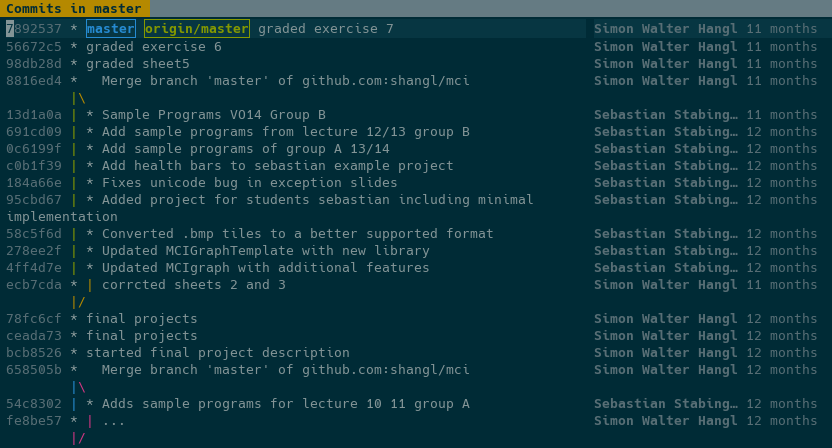
\includegraphics[width=1.0\textwidth]{img/screenshot-20180608-171423.png}
\end{center}\end{center}
\end{frame}
\begin{frame}[label={sec:org2c17d14}]{Übersichtlicher}
\begin{itemize}
\item Es ist wesentlich einfacher bestimmte Teile eines Programms zu
finden wenn mehrere Dateien verwendet werden
\item Wenn z.B. jede Klasse in einer eigenen Datei liegt findet man diese
sehr einfach über den Klassennamen
\item Mit einer modernen IDE ist das kein so großes Problem mehr wie früher
\begin{itemize}
\item Es gibt z.B. üblicherweise eine eigene Klassenansicht die
unabhängig von Dateien arbeitet
\item Es kommt aber immer wieder vor, dass man ohne IDE auskommen muss,
oder externe Tools verwendet werden die mit einer Aufteilung auf
Dateien übersichtlicher werden
\end{itemize}
\end{itemize}
\end{frame}
\begin{frame}[label={sec:org2421e86}]{Compilezeiten}
\begin{itemize}
\item Große Projekte können \alert{Stunden} für einen kompletten Compilevorgang
benötigen. Daduch kann das Programmieren extrem ineffizient werden
\item Wenn ein Programm auf mehrere Dateien aufgeteilt ist müssen nur die
Dateien neu compiliert werden die sich \alert{geändert} haben
\end{itemize}
\begin{center}\begin{center}
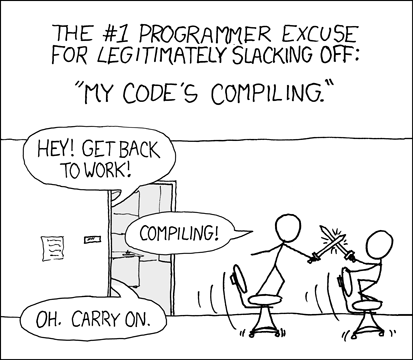
\includegraphics[width=0.5\textwidth]{img/compiling.png}
\end{center}\end{center}
\tiny \center
\url{https://xkcd.com/303/}
\end{frame}
\section{Wie teilt man Programme auf mehrere Dateien auf?}
\label{sec:org06e1dcc}
\begin{frame}[label={sec:org64a79e6},fragile]{Das generelle Prinzip}
 \begin{itemize}
\item Wir wollen also Teile unseres Programms aus der Hauptdatei (in der
die {\color{solarizedYellow}\texttt{main}}--Funktion liegt) auslagern
\item In C/C++ müssen für ausgelagerte Teile immer zwei Dateien
geschrieben werden. Die \alert{Headerdatei} und die eigentliche
\alert{Quellcodedatei}
\end{itemize}
\begin{block}{Headerdatei}
Definiert \alert{welche Funktionalität} der ausgelagerte Teil anbietet. z.B.
Funktionen und Klassen
\end{block}
\begin{block}{Quellcodedatei}
\alert{Implementiert} die in der Headerdatei definierte Funktionalität
\end{block}
\end{frame}
\begin{frame}[label={sec:org493deab},fragile]{Die Headerdatei}
 \begin{itemize}
\item Enthält einen sogenannten \alert{Include Guard} der verhindert, dass die
selbe Headerdatei öfter als ein mal inkludiert werden kann
\item Enthält \alert{Signaturen} aller Funktionen und Klassen
\item Enthält Namen von \alert{Konstanten} und \alert{globalen Variablen}
\item Enthält {\color{solarizedYellow}\texttt{\#include} }für anderen Headerdateien
\end{itemize}
\begin{block}{Include Guard}
\begin{minted}[fontsize=\scriptsize,numberblanklines=false]{c++}
#ifndef EINDEUTIGER_NAME
#define EINDEUTIGER_NAME

// Alles andere kommt hier hin!

#endif
\end{minted}
\end{block}
\begin{block}{Signaturen?}
Signaturen teilen dem Compiler mit welche Funktionen und Klassen es
gibt, ohne die Funktionalität bereits zu implementieren
\end{block}
\end{frame}
\begin{frame}[label={sec:orgd2a97c8},fragile]{Was macht {\color{solarizedYellow}\texttt{\#include} }eigentlich?}
 \begin{itemize}
\item {\color{solarizedYellow}\texttt{\#include} }ersetzt die Zeile in der {\color{solarizedYellow}\texttt{\#include} }steht mit dem Inhalt
der angegebenen Datei
\item Der \alert{Include Guard} verhindert, dass der Inhalt einer Datei nicht
öfters verwendet wird.
\end{itemize}
\begin{block}{Beispiel}
\begin{minted}[fontsize=\scriptsize,numberblanklines=false]{c++}
#include <iostream>
#include <iostream>
#include <iostream>
\end{minted}
Die wiederholten Einfügungen von {\color{solarizedYellow}\texttt{iostream} }werden vor dem compilieren
wieder gelöscht.
\end{block}
\end{frame}

\begin{frame}[label={sec:orga76bc22},fragile]{Signaturen von Funktionen}
 Bestehen einfach aus dem \alert{Teil einer Funktion vor den {\color{solarizedYellow}\texttt{\{ \}}}}
\begin{block}{Beispiele}
\begin{minted}[fontsize=\scriptsize,numberblanklines=false]{c++}
int add(int a, int b);
bool is_even(int number);
void print_my_stuff(MyClass &c);
// ...
\end{minted}
\end{block}
\begin{block}{Parameternamen}
Die Signatur einer Funktion muss prinzipiell \alert{keine Parameternamen}
enthalten. Es ist für den Compiler nur wichtig, dass die Typen alle
korrekt sind:
\begin{minted}[fontsize=\scriptsize,numberblanklines=false]{c++}
int add(int, int);
bool is_even(int);
void print_my_stuff(MyClass &);
// ...
\end{minted}
Der Übersichtlichkeit halber \alert{verwendet man sie generell aber trotzdem}!
\end{block}
\end{frame}
\begin{frame}[label={sec:org4a15753},fragile]{Signaturen von Klassen}
 Die Signatur einer Klasse ist aufgebaut wie eine Klasse die wir bis
jetzt gesehen haben, \alert{enthält aber statt der Funktionen nur die
Funktionssignaturen}.
\begin{block}{Beispiel für die ursprüngliche Player Klasse}
\begin{minted}[fontsize=\scriptsize,numberblanklines=false]{c++}
class Player {
private:
    int _posx, _posy;      
    string _img;           
    int _fieldsx, _fieldsy;
    int _sizex, _sizey;    

public:
    Player(int posx, int posy, string img, int fieldsx,
           int fieldsy, int sizex, int sizey);

    void move_left();
    void move_right();
    void move_up();
    void move_down();
    void draw();
};
\end{minted}
\end{block}
\end{frame}
\begin{frame}[label={sec:org60aae87},fragile]{Die Quellcodedatei}
 \begin{itemize}
\item Inkludiert die zuvor beschriebene Headerdatei mit {\color{solarizedYellow}\texttt{\#include
  "dateiname.h"} }(\alert{Achtung:} Die Anführungszeichen sind wichtig!)
\item Implementiert die Funktionen und die Memberfunktionen von Klassen
die wir in der Headerdatei beschrieben haben (siehe die folgenden
beiden Beispiele)
\end{itemize}
\end{frame}
\begin{frame}[label={sec:org34f4890},fragile]{Auslagern von Funktionen --- Beispiel}
 Wir wollen {\color{solarizedYellow}\texttt{is\_prime} }des folgenden Programms auslagern:

\noindent\rule{\textwidth}{0.5pt}
\begin{minted}[fontsize=\scriptsize,numberblanklines=false]{c++}
#include <iostream>
using namespace std;

bool is_prime(int number) {
  for (int i = 2; i < number / 2 + 1; i++) {
    if (number % i == 0)
      return false;
  }
  return true;
}

int main() {
  for (int i = 2; i < 100; i++) {
    if (is_prime(i)) {
      cout << i << " ist eine Primzahl" << endl;
    }
  }
}
\end{minted}
\end{frame}
\begin{frame}[label={sec:org645b907},fragile]{Auslagern von Funktionen --- Beispiel}
 \begin{block}{prime.hpp}
\begin{minted}[fontsize=\scriptsize,numberblanklines=false]{c++}
#ifndef PRIME_H
#define PRIME_H

bool is_prime(int number);

#endif /* PRIME_H */
\end{minted}
\end{block}
\begin{block}{prime.cpp}
\begin{minted}[fontsize=\scriptsize,numberblanklines=false]{c++}
#include "prime.hpp"

bool is_prime(int number) {
    for (int i = 2; i < number / 2 + 1; i++) {
        if (number % i == 0)
            return false;
    }
    return true;
}
\end{minted}
\end{block}
\end{frame}
\begin{frame}[label={sec:org69033c4},fragile]{Auslagern von Funktionen --- Beispiel}
 \begin{block}{main.cpp}
\begin{minted}[fontsize=\scriptsize,numberblanklines=false]{c++}
#include <iostream>
#include "prime.hpp"
using namespace std;

int main() {
  for (int i = 2; i < 100; i++) {
    if (is_prime(i)) {
      cout << i << " ist eine Primzahl" << endl;
    }
  }
}
\end{minted}
\end{block}
\end{frame}

\begin{frame}[label={sec:org179425b},fragile]{Auslagern von Klassen --- Beispiel}
 Wir wollen {\color{solarizedYellow}\texttt{Average} }des folgenden Programms auslagern:
\begin{minted}[fontsize=\scriptsize,numberblanklines=false]{c++}
#include <iostream>
using namespace std;

class Average {
private:
    double sum = 0.0;
    int count = 0;

public:
    void add(double val) {
        sum += val;
        count++;
    }

    double get_avg() { return sum / count; }
};

int main() {
  Average avg;
  avg.add(12.3);
  avg.add(11.7);
  avg.add(13.7);
  cout << avg.get_avg() << endl;
}
\end{minted}
\end{frame}
\begin{frame}[label={sec:org6fa125c},fragile]{Auslagern von Klassen --- Beispiel}
 \begin{block}{average.hpp}
\begin{minted}[fontsize=\scriptsize,numberblanklines=false]{c++}
#ifndef AVERAGE_H
#define AVERAGE_H

class Average {
private:
    double sum = 0.0;
    int count = 0;

public:
    void add(double val);
    double get_avg();
};

#endif /* AVERAGE_H */
\end{minted}
\end{block}
\end{frame}
\begin{frame}[label={sec:org256b9ce},fragile]{Auslagern von Klassen --- Beispiel}
 \begin{block}{average.cpp}
\begin{minted}[fontsize=\scriptsize,numberblanklines=false]{c++}
#include "average.hpp"

void Average::add(double val) {
    sum += val;
    count++;
}

double Average::get_avg() { return sum / count; }
\end{minted}
\end{block}
\begin{block}{main.cpp}
\begin{minted}[fontsize=\scriptsize,numberblanklines=false]{c++}
#include "average.hpp"
#include <iostream>
using namespace std;

int main() {
  Average avg;
  avg.add(12.3);
  avg.add(11.7);
  avg.add(13.7);
  cout << avg.get_avg() << endl;
}
\end{minted}
\end{block}
\end{frame}
\begin{frame}[label={sec:org5684781},fragile]{Globale Variablen}
 Globale Variablen müssen in der Headerdatei mit {\color{solarizedYellow}\texttt{extern} }markiert und
in der Quellcodedatei erzeugt werden
\begin{block}{Header}
\begin{minted}[fontsize=\scriptsize,numberblanklines=false]{c++}
// ...
extern int meine_globale_variable;
// ...
\end{minted}
\end{block}
\begin{block}{Quellcodedatei}
\begin{minted}[fontsize=\scriptsize,numberblanklines=false]{c++}
#include "header.hpp"
int meine_globale_variable = 42;
\end{minted}
\end{block}
\begin{block}{Main}
\begin{minted}[fontsize=\scriptsize,numberblanklines=false]{c++}
#include "header.cpp"
#include <iostream>

int main() { 
  std::cout << meine_globale_variable << std::endl; 
}
\end{minted}
\end{block}
\end{frame}
\begin{frame}[label={sec:org7330903},fragile]{Übung}
 \begin{itemize}
\item Laden Sie sich die Datei {\color{solarizedYellow}\texttt{split\_off.cpp} }aus Sakai
\item Lagern Sie alles bis auf die {\color{solarizedYellow}\texttt{main}}-Funktion in eine Header- und
Quellcodedatei aus
\end{itemize}
\end{frame}
\end{document}